\documentclass[fontsize=11pt,reqno,a4paper,oneside]{scrartcl}

% ---- Sprache und Textformatierung ----
\usepackage{fontspec}
\usepackage{polyglossia}
\setdefaultlanguage{english}   
\usepackage{csquotes}
\usepackage{acronym}

% ---- KOMA-Script Seiteneinstellungen ----
\usepackage[onehalfspacing]{setspace}  
\usepackage[headsepline]{scrlayer-scrpage}

% Kopfzeilen-Konfiguration
\clearpairofpagestyles  % Alle bestehenden Kopf- und Fußzeilen löschen
\addtokomafont{pagehead}{\normalfont\small}  % Schriftart der Kopfzeile
\automark[section]{section}
\ihead{\textsc{\headmark}} 
\cfoot{\pagemark}

% ---- Mathematik und Symbole ----
\usepackage{amsmath, amsthm, amssymb, mathtools}
\usepackage[version=4]{mhchem}
\usepackage{chemformula}
\newcommand{\angstrom}{\text{\normalfont\AA}}

% ---- Graphische Pakete ----
\usepackage{xcolor}
\usepackage{graphicx}
\usepackage{float}
\usepackage{siunitx}
\usepackage{textpos}
\usepackage{subfig}
\usepackage{svg}

% ---- Text-Positionierung ----
\usepackage[pscoord]{eso-pic}
\newcommand{\placetextbox}[3]{% \placetextbox{<horizontal pos>}{<vertical pos>}{<stuff>}
  \setbox0=\hbox{#3}% Put <stuff> in a box
  \AddToShipoutPictureFG*{% Add <stuff> to current page foreground
    \put(\LenToUnit{#1\paperwidth},\LenToUnit{#2\paperheight}){\vtop{{\null}\makebox[0pt][c]{#3}}}%
  }%
}%

% ---- Bibliographie ----
\usepackage[backend=biber,
    citestyle=numeric-comp,
    bibstyle=numeric,
    bibwarn=true,
    autocite=superscript,
    abbreviate=true, 
    sorting=none, 
    url=false, 
    doi=false,
    eprint=false,
    isbn=false]{biblatex}

% Definition eines neuen Zitierbefehls mit eckigen Klammern
\DeclareCiteCommand{\supercite}[\mkbibsuperscript]%
    {\usebibmacro{cite:init}%
        \let\multicitedelim\supercitedelim%
        \iffieldundef{prenote}%
        {}%
        {\BibliographyWarning{Ignoring prenote argument}}%
        \iffieldundef{postnote}%
        {}%
        {\BibliographyWarning{Ignoring postnote argument}}%
        \bibleftbracket}%
    {\usebibmacro{citeindex}%
        \usebibmacro{cite:comp}}
    {}%
    {\usebibmacro{cite:dump}%
        \bibrightbracket}

% Bibliographie-Dateien
\addbibresource{/Users/lucashirschfeld/sciebo/VsCode/LaTeX-Projects/bibliography/zotero.bib}

% ---- Hyperlinks ----
\usepackage{hyperref}
\hypersetup{colorlinks=true, linkcolor=black, citecolor=black, urlcolor=black}

% ---- Dokumenteinstellungen ----
\setlength{\parindent}{0pt}

% ---- Metadaten ----
\def\Autor{Lucas Hirschfeld, s6luhirs@uni-bonn.de}
\def\Titel{\ac{TDS} of Phenol on the Ag(111) surface}
\def\Date{First Submission: \today}
\def\PiC{Supervisor: Anna Juliana Kny}
\def\Abstract{} 

\begin{document}
\pagestyle{empty}
\begin{titlepage}
    \begin{center}
        \vspace*{\fill}
        {\LARGE\bfseries \Titel}\par\vspace{2cm}
        {\Autor\par\vspace{0.5cm}\PiC\par\vspace{1cm}\par\vspace{0.2cm}\Date\par\vspace{5cm}}
    \end{center}
    {\Abstract\vspace{0.5cm}\par}\vfill
\end{titlepage}

\pagestyle{scrheadings}
\tableofcontents
\pagenumbering{arabic}
\clearpage

\section{Introduction}

\clearpage
\section{Experimental}

\clearpage
\section{Results}

\subsection{Residual gas analysis}

\begin{figure}
    \centering
    
\includegraphics[width=0.9\textwidth]{images/residual gas_3_plot.pdf}
    \caption{Residual gas analysis of the UHV chamber.}
    \label{fig:rga_normal}
\end{figure}

\begin{figure}
    \centering
    
\includegraphics[width=0.9\textwidth]{images/residual gas_4_plot.pdf}
    \caption{Residual gas analysis of the UHV chamber with argon.}
    \label{fig:rga_argon}
\end{figure}

\begin{figure}
    \centering
    
\includegraphics[width=0.9\textwidth]{images/residual gas_8_plot.pdf}
    \caption{Residual gas analysis of the UHV chamber while degasing the filament.}
    \label{fig:rga_filament}
\end{figure}

\clearpage
\subsection{Mass Spectra for Phenol and Benzene}

\begin{figure}
    \centering
    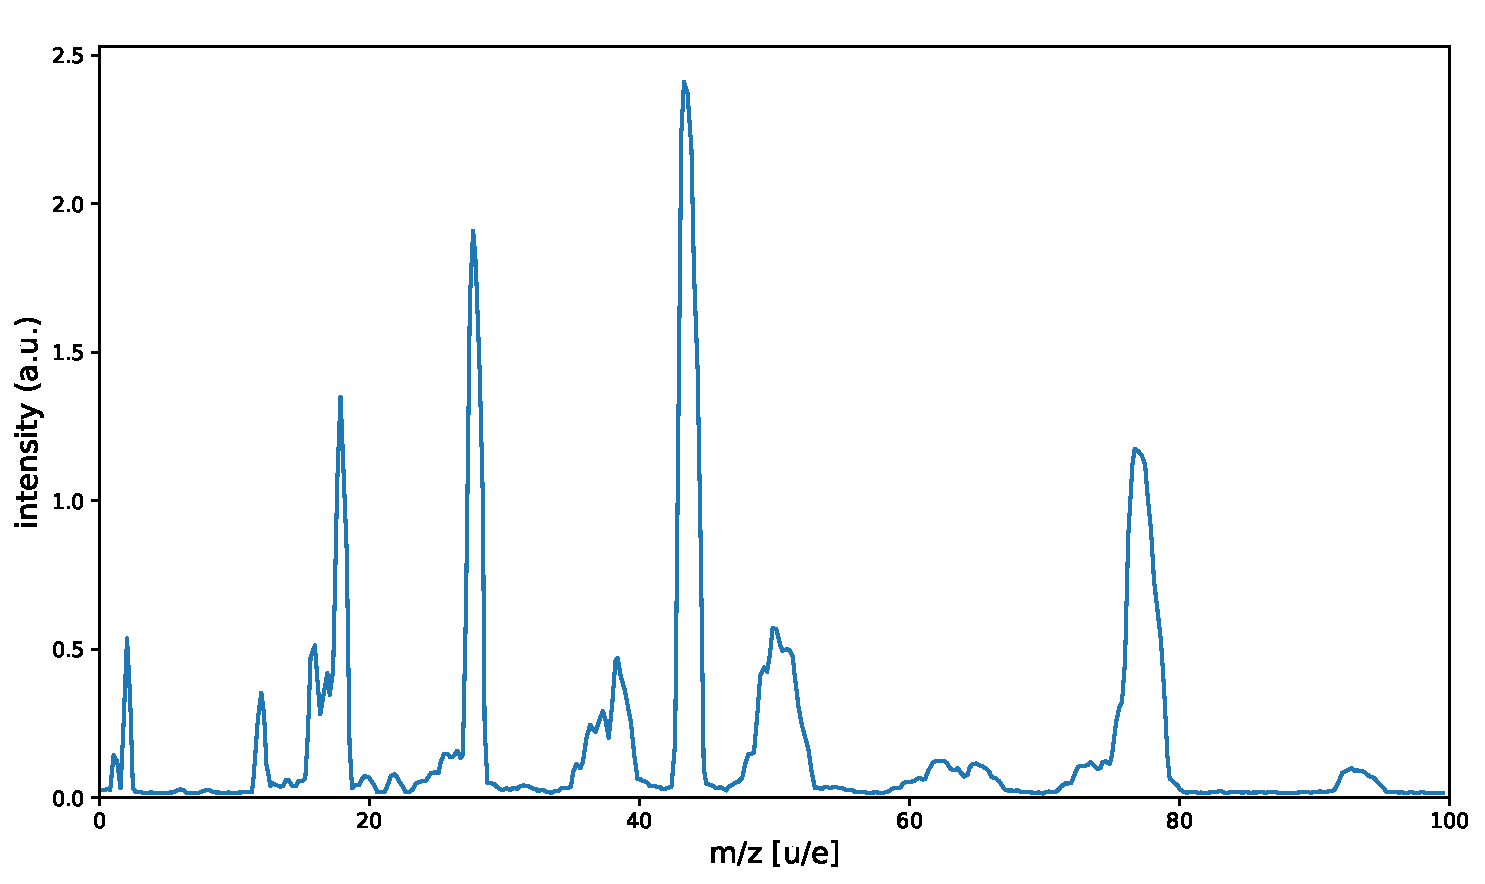
\includegraphics[width=0.9\textwidth]{images/Mass spectra_Benzen_plot.pdf}
    \caption{Mass spectrum of benzene.}
    \label{fig:benzene_mass_spectrum}
\end{figure}

\begin{figure}
    \centering
    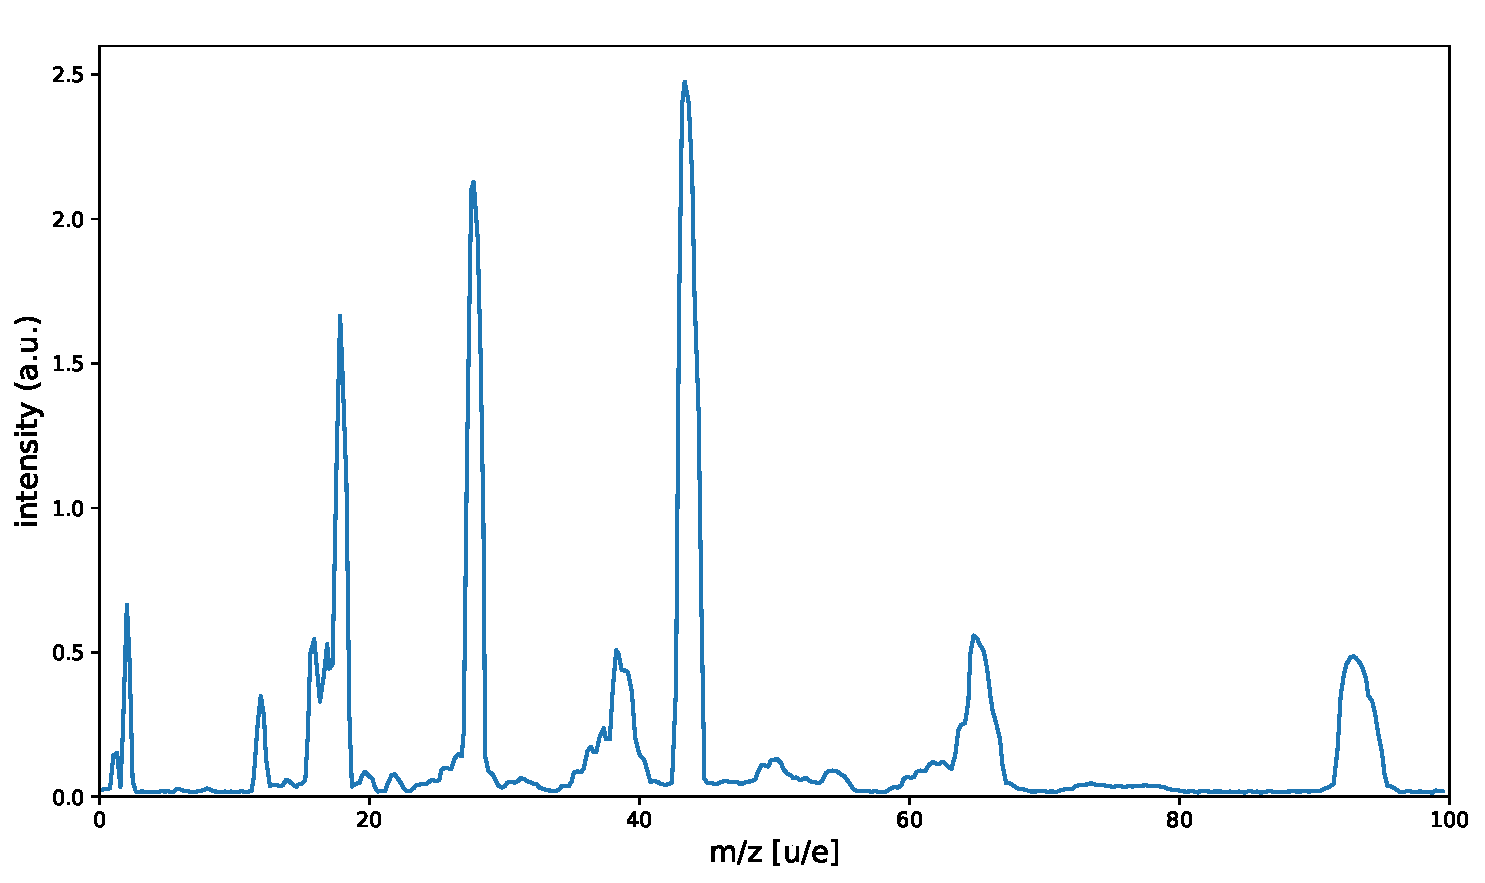
\includegraphics[width=0.9\textwidth]{images/Mass spectra_Phenol_plot.pdf}
    \caption{Mass spectrum of phenol.}
    \label{fig:phenol_mass_spectrum}
\end{figure}

\clearpage
\subsection{TDS Spectra of Phenol on Ag(111)}

\begin{figure}
    \centering
    
\includegraphics[width=0.9\textwidth]{images/phenol_TPD_spectra_sorted_by_dosage.pdf}
    \caption{\ac{TDS} spectrum of phenol on Ag(111) with different coverages.}
    \label{fig:tds_phenol_all}
\end{figure}

\subsection{Geometric Model of the Monolayer}

\begin{figure}
    \centering
    
\includegraphics[width=0.9\textwidth]{images/phenol_TPD_1ML.pdf}
    \caption{\ac{TDS} spectrum of 1~\ac{ML} of phenol on Ag(111).}
    \label{fig:phenol_TPD_1ML}
\end{figure}

\clearpage
\subsection{Behavior of Coverage and Dosage}

\begin{table}
    \centering
    \caption{Dosage, integral of the TDS spectra and coverage for phenol on Ag(111). The coverage is calculated from the \ac{TDS} spectra.}
    \begin{tabular}{|c|c|c|c|}
        \hline
        Dosage [mbar s] & Integral range [K] & Integral [a.u.] & Coverage [ML] \\
        \hline
        $1.70 \cdot 10^{-8}$ & 155-270 & $9.08 \cdot 10^{0}$ & 0.22 \\
        $1.40 \cdot 10^{-7}$ & 155-270 & $2.27 \cdot 10^{1}$ & 0.54 \\
        $1.70 \cdot 10^{-7}$ & 155-270 & $2.88 \cdot 10^{1}$ & 0.69 \\
        $2.10 \cdot 10^{-7}$ & 155-270 & $4.02 \cdot 10^{1}$ & 0.96 \\
        $2.40 \cdot 10^{-7}$ & 155-270 & $4.17 \cdot 10^{1}$ & 1.00 \\
        $2.80 \cdot 10^{-7}$ & 155-270 & $5.02 \cdot 10^{1}$ & 1.20 \\
        $3.80 \cdot 10^{-7}$ & 155-268 & $6.20 \cdot 10^{1}$ & 1.49 \\
        $4.10 \cdot 10^{-7}$ & 155-265 & $5.72 \cdot 10^{1}$ & 1.37 \\
        $7.50 \cdot 10^{-7}$ & 155-260 & $1.19 \cdot 10^{2}$ & 2.84 \\
        $1.00 \cdot 10^{-6}$ & 155-258 & $1.66 \cdot 10^{2}$ & 3.97 \\
        $1.40 \cdot 10^{-6}$ & 155-258 & $1.65 \cdot 10^{2}$ & 3.95 \\
        \hline
    \end{tabular}
    \label{tab:phenol_coverage_and_dosage}
\end{table}


\begin{figure}
    \centering
    
\includegraphics[width=0.9\textwidth]{images/phenol_TPD_coverage_vs_dosage.pdf}
    \caption{Coverage as a function of dosage for phenol on Ag(111). The coverage is calculated from the \ac{TDS} spectra.}
    \label{fig:coverage_and_dosage}
\end{figure}

\clearpage
\subsection{Sticking Factor}

\begin{figure}
    \centering
    \subfloat[p(2×2) model]{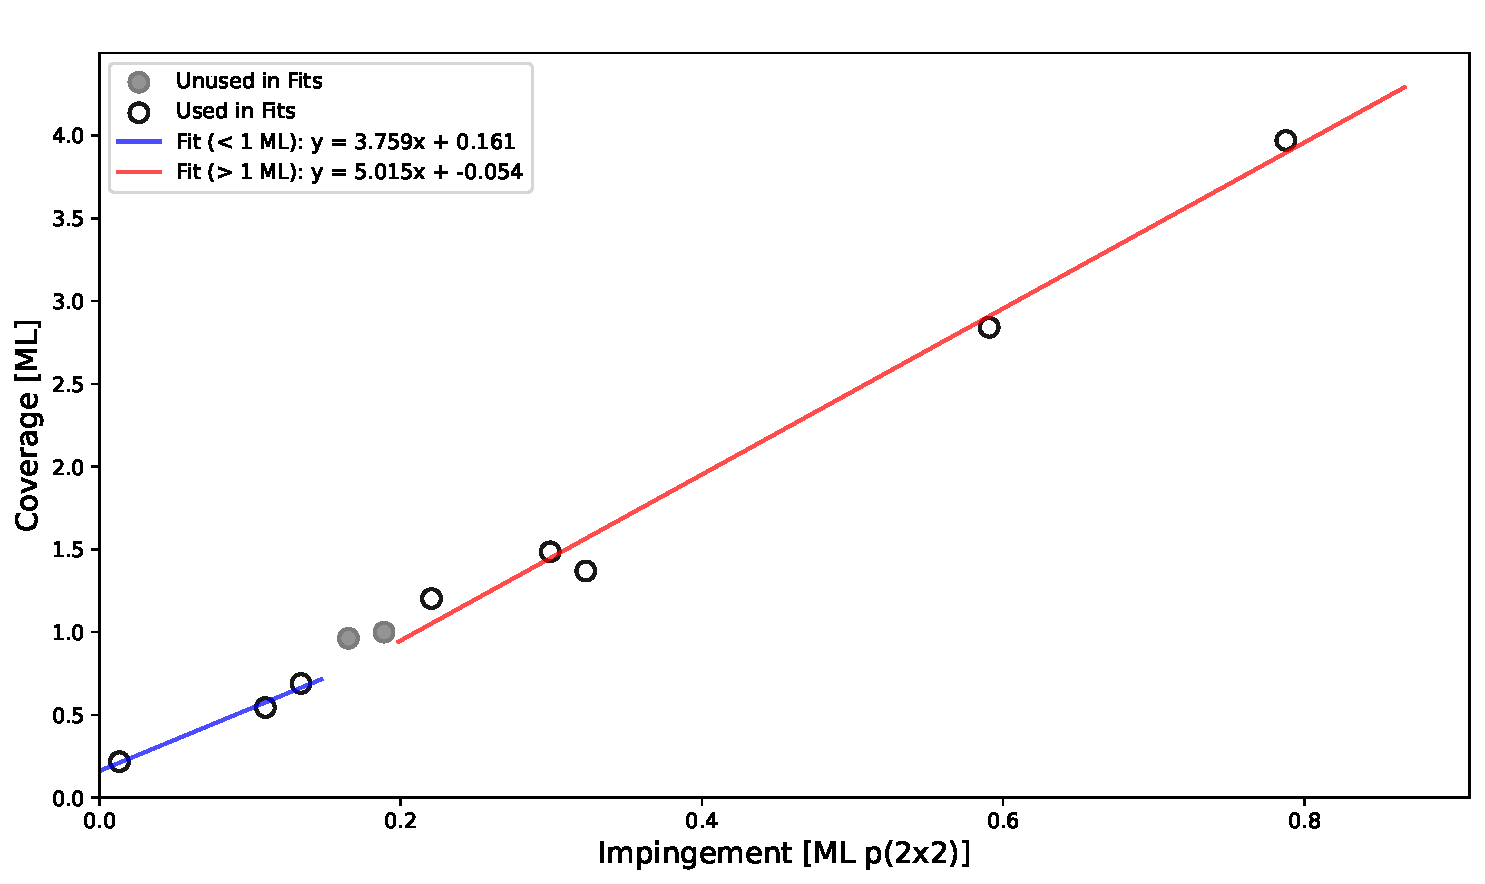
\includegraphics[width=0.6\textwidth]{images/phenol_TPD_coverage_vs_impingement_p2x2.pdf}\label{fig:impingement_p2x2}}
    \hfill
    \subfloat[p(4×4) model]{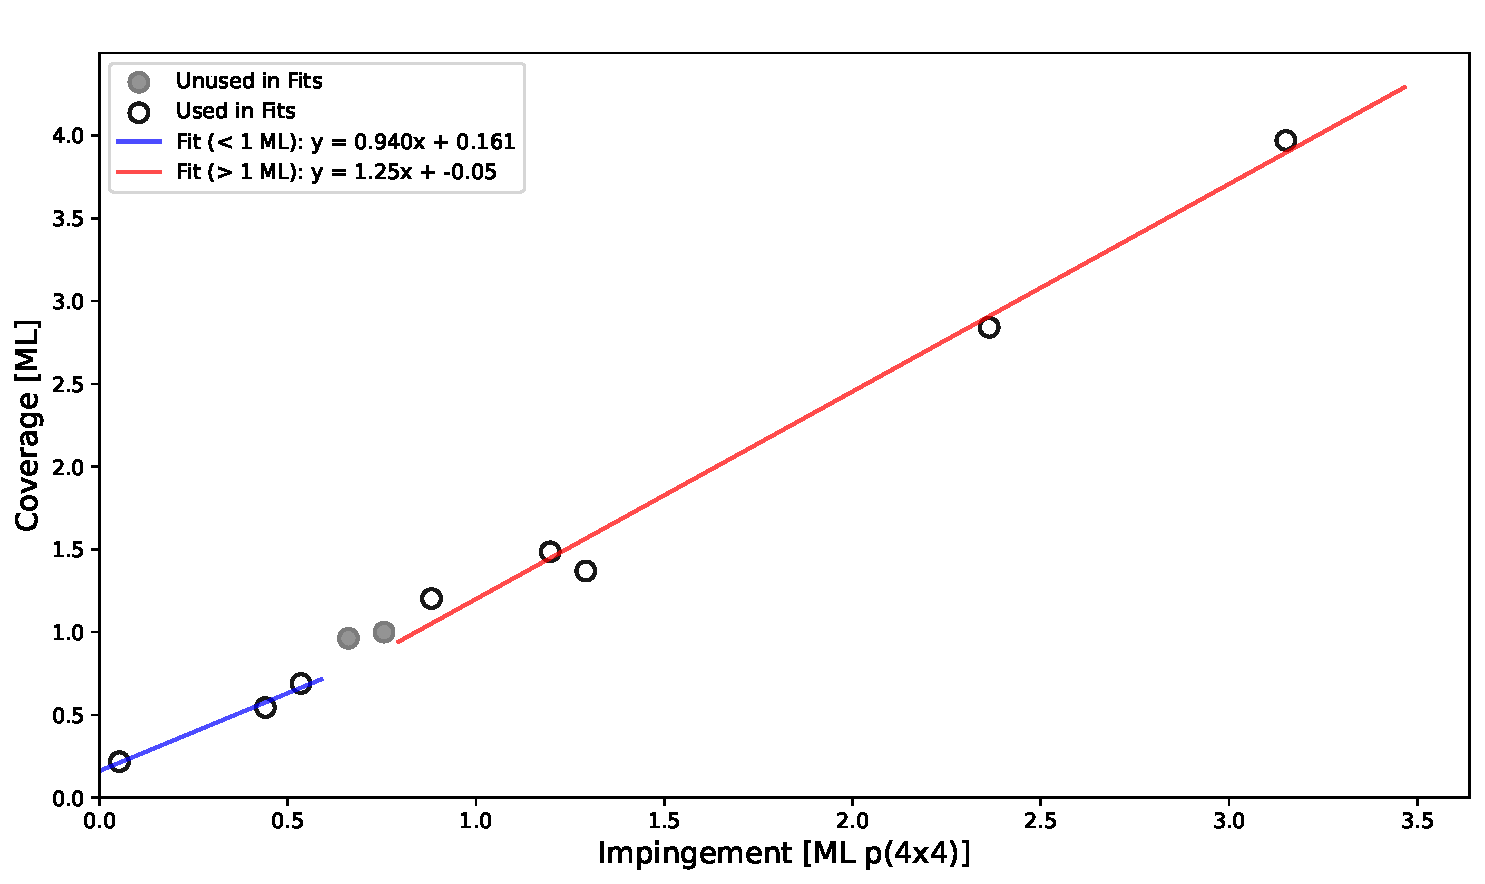
\includegraphics[width=0.6      \textwidth]{images/phenol_TPD_coverage_vs_impingement_p4x4.pdf}\label{fig:impingement_p4x4}}
    \hfill
    \subfloat[p(6×6) model]{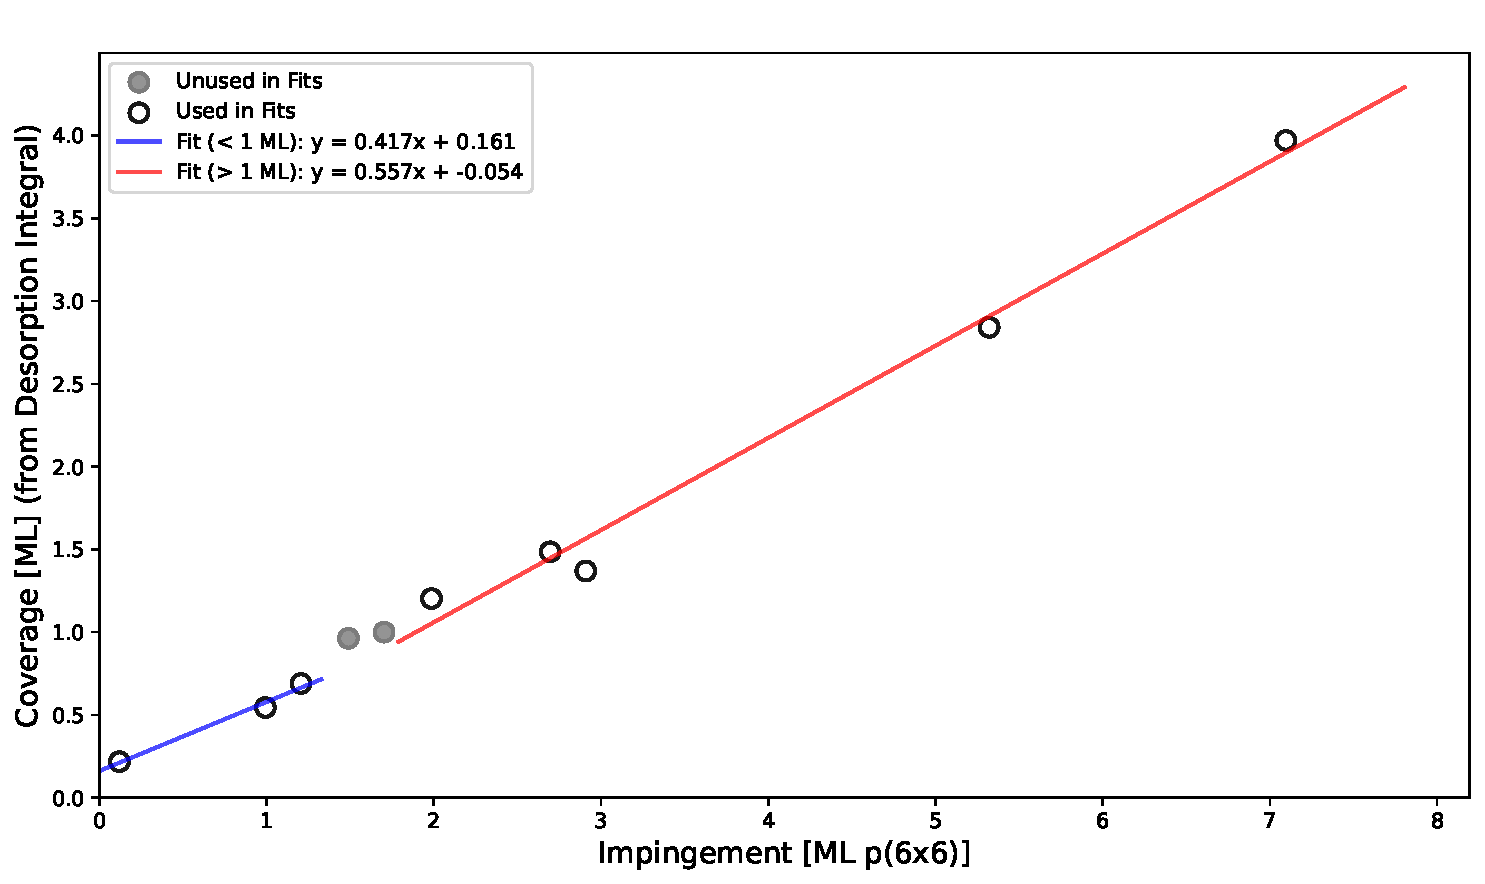
\includegraphics[width=0.6\textwidth]{images/phenol_TPD_coverage_vs_impingement_p6x6.pdf}\label{fig:impingement_p6x6}}
    \caption{Coverage as a function of impingement rate for phenol on Ag(111) with different geometric models.}
    \label{fig:impingement_models}
\end{figure}

\begin{table}
    \centering
    \caption{Dosage, coverage, and impingement rate for phenol on Ag(111).}
    \begin{tabular}{|c|c|c|}
        \hline
        Dosage $D$ [mbar s] & Coverage $\theta$ [ML] & $N_\mathrm{imp}$ [cm$^{-2}$] \\
        \hline
        $1.70 \cdot 10^{-8}$ & 0.22 & $4.62 \cdot 10^{12}$ \\
        $1.40 \cdot 10^{-7}$ & 0.54 & $3.80 \cdot 10^{13}$ \\
        $1.70 \cdot 10^{-7}$ & 0.69 & $4.62 \cdot 10^{13}$ \\
        $2.10 \cdot 10^{-7}$ & 0.96 & $5.71 \cdot 10^{13}$ \\
        $2.40 \cdot 10^{-7}$ & 1.00 & $6.52 \cdot 10^{13}$ \\
        $2.80 \cdot 10^{-7}$ & 1.20 & $7.61 \cdot 10^{13}$ \\
        $3.80 \cdot 10^{-7}$ & 1.49 & $1.03 \cdot 10^{14}$ \\
        $4.10 \cdot 10^{-7}$ & 1.37 & $1.11 \cdot 10^{14}$ \\
        $7.50 \cdot 10^{-7}$ & 2.84 & $2.04 \cdot 10^{14}$ \\
        $1.00 \cdot 10^{-6}$ & 3.97 & $2.72 \cdot 10^{14}$ \\
        $1.40 \cdot 10^{-6}$ & 3.95 & $3.80 \cdot 10^{14}$ \\
        \hline
    \end{tabular}
    \label{tab:dosage_coverage_impingement}
\end{table}

\clearpage
\subsection{Desorption Energy and Pre-Exponential Factor for the Multilayer}

\begin{figure}
    \centering
    
\includegraphics[width=0.9\textwidth]{images/phenol_TPD_arrhenius_plot.pdf}
    \caption{Menzel-Schlichting plot for the multilayer of phenol on Ag(111). The desorption energy is calculated from the slope and the pre-exponential factor is calculated from the intercept of the Menzel-Schlichting plot.}
    \label{fig:Menzel_Schlichting_plot}
\end{figure}

\begin{table}
    \centering
    \caption{Desorption parameters from Menzel-Schlichting analysis for phenol on Ag(111).}
    \begin{tabular}{|c|c|c|}
        \hline
        Coverage $\theta$ [ML] & Desorption Energy $E$ [kJ/mol] & Pre-exponential Factor $\nu$ [s$^{-1}$] \\
        \hline
        2.84 & $52.0\pm0.4$ & $(2.27\pm0.57) \cdot 10^{14}$ \\
        3.97 & $50.8\pm0.2$ & $(1.24\pm0.20) \cdot 10^{14}$ \\
        3.95 & $55.2\pm0.2$ & $(2.82\pm0.32) \cdot 10^{15}$ \\
        \hline
    \end{tabular}
    \label{tab:menzel_schlichting_parameters}
\end{table}

\clearpage
\subsection{Monolayer Desorption}



\clearpage
\section{Discussion}



\clearpage
\section{Appendix}

\subsection*{Acronyms}

\begin{acronym}
    \acro{TDS}[TDS]{Thermal desorption spectroscopy}
\end{acronym}

\printbibliography[heading=bibintoc, title={References}] 

\end{document}